\subsection*{Тест 1}

Параметры тестирования:

\begin{itemize}
    \item Количество операций: 32
    \item Вероятность выполнения операции \verb|add|: 33.33 \%
    \item Вероятность выполнения операции \verb|remove|: 33.33 \%
    \item Вероятность выполнения операции \verb|contains|: 33.33 \%
\end{itemize}

Результаты тестирования представленны в таблице \ref{tab:results1}


\begin{table}[H]
    \centering
    \begin{tabular}{|l|l|}
        \hline
        Кол-во потоков & Время выполнения (мс) \\
        \hline
        1 & 11 \\
        \hline
        2 & 10 \\
        \hline
        3 & 12 \\
        \hline
        4 & 4 \\
        \hline
    \end{tabular}
    \caption{Результаты теста 1}
    \label{tab:results1}
\end{table}
        

График результатов тестирования представлен на рис.\ref{fig:plot1}

\begin{figure}[H]
    \centering
    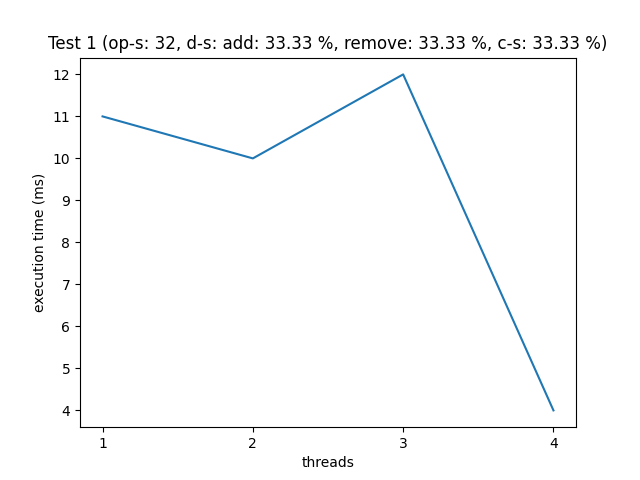
\includegraphics[width=0.7\linewidth]{photo/plot1}
    \caption{График результатов теста 1}
    \label{fig:plot1}
\end{figure}

\subsection*{Тест 2}

Параметры тестирования:

\begin{itemize}
    \item Количество операций: 32
    \item Вероятность выполнения операции \verb|add|: 90 \%
    \item Вероятность выполнения операции \verb|remove|: 9 \%
    \item Вероятность выполнения операции \verb|contains|: 1 \%
\end{itemize}

Результаты тестирования представленны в таблице \ref{tab:results2}


\begin{table}[H]
    \centering
    \begin{tabular}{|l|l|}
        \hline
        Кол-во потоков & Время выполнения (мс) \\
        \hline
        1 & 2 \\
        \hline
        2 & 3 \\
        \hline
        3 & 8 \\
        \hline
        4 & 15 \\
        \hline
    \end{tabular}
    \caption{Результаты теста 2}
    \label{tab:results2}
\end{table}
        

График результатов тестирования представлен на рис.\ref{fig:plot2}

\begin{figure}[H]
    \centering
    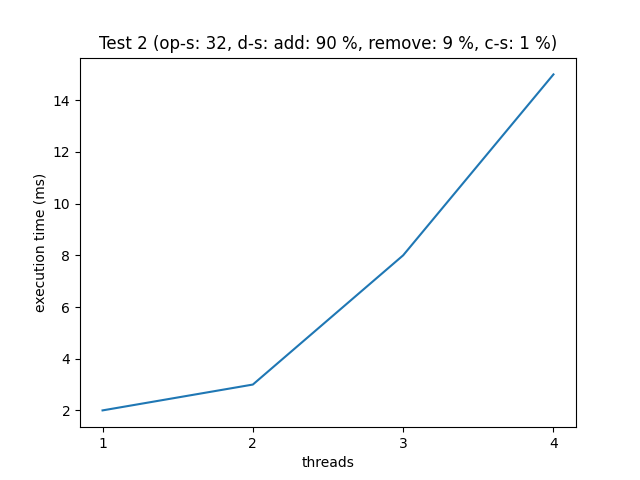
\includegraphics[width=0.7\linewidth]{photo/plot2}
    \caption{График результатов теста 2}
    \label{fig:plot2}
\end{figure}

\subsection*{Тест 3}

Параметры тестирования:

\begin{itemize}
    \item Количество операций: 32
    \item Вероятность выполнения операции \verb|add|: 90 \%
    \item Вероятность выполнения операции \verb|remove|: 1 \%
    \item Вероятность выполнения операции \verb|contains|: 9 \%
\end{itemize}

Результаты тестирования представленны в таблице \ref{tab:results3}


\begin{table}[H]
    \centering
    \begin{tabular}{|l|l|}
        \hline
        Кол-во потоков & Время выполнения (мс) \\
        \hline
        1 & 8 \\
        \hline
        2 & 8 \\
        \hline
        3 & 11 \\
        \hline
        4 & 9 \\
        \hline
    \end{tabular}
    \caption{Результаты теста 3}
    \label{tab:results3}
\end{table}
        

График результатов тестирования представлен на рис.\ref{fig:plot3}

\begin{figure}[H]
    \centering
    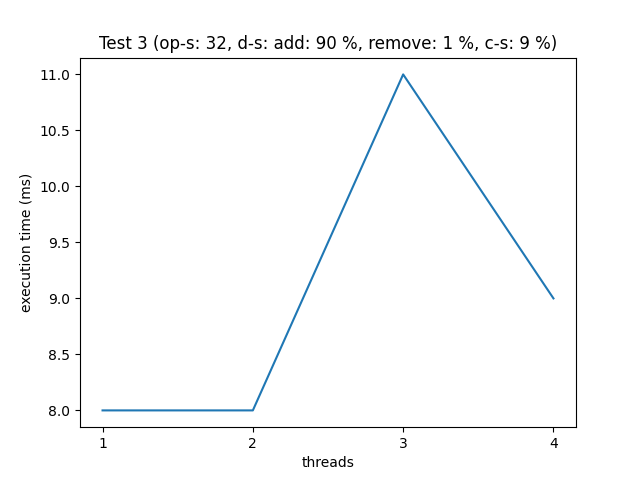
\includegraphics[width=0.7\linewidth]{photo/plot3}
    \caption{График результатов теста 3}
    \label{fig:plot3}
\end{figure}

\subsection*{Тест 4}

Параметры тестирования:

\begin{itemize}
    \item Количество операций: 32
    \item Вероятность выполнения операции \verb|add|: 9 \%
    \item Вероятность выполнения операции \verb|remove|: 90 \%
    \item Вероятность выполнения операции \verb|contains|: 1 \%
\end{itemize}

Результаты тестирования представленны в таблице \ref{tab:results4}


\begin{table}[H]
    \centering
    \begin{tabular}{|l|l|}
        \hline
        Кол-во потоков & Время выполнения (мс) \\
        \hline
        1 & 6 \\
        \hline
        2 & 14 \\
        \hline
        3 & 18 \\
        \hline
        4 & 18 \\
        \hline
    \end{tabular}
    \caption{Результаты теста 4}
    \label{tab:results4}
\end{table}
        

График результатов тестирования представлен на рис.\ref{fig:plot4}

\begin{figure}[H]
    \centering
    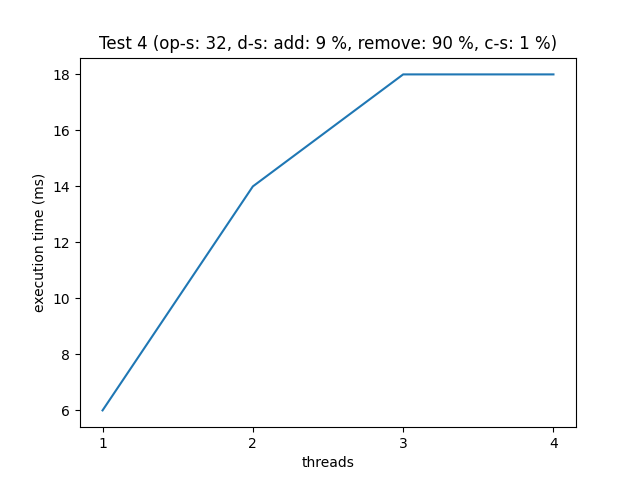
\includegraphics[width=0.7\linewidth]{photo/plot4}
    \caption{График результатов теста 4}
    \label{fig:plot4}
\end{figure}

\subsection*{Тест 5}

Параметры тестирования:

\begin{itemize}
    \item Количество операций: 32
    \item Вероятность выполнения операции \verb|add|: 1 \%
    \item Вероятность выполнения операции \verb|remove|: 90 \%
    \item Вероятность выполнения операции \verb|contains|: 9 \%
\end{itemize}

Результаты тестирования представленны в таблице \ref{tab:results5}


\begin{table}[H]
    \centering
    \begin{tabular}{|l|l|}
        \hline
        Кол-во потоков & Время выполнения (мс) \\
        \hline
        1 & 1 \\
        \hline
        2 & 1 \\
        \hline
        3 & 2 \\
        \hline
        4 & 2 \\
        \hline
    \end{tabular}
    \caption{Результаты теста 5}
    \label{tab:results5}
\end{table}
        

График результатов тестирования представлен на рис.\ref{fig:plot5}

\begin{figure}[H]
    \centering
    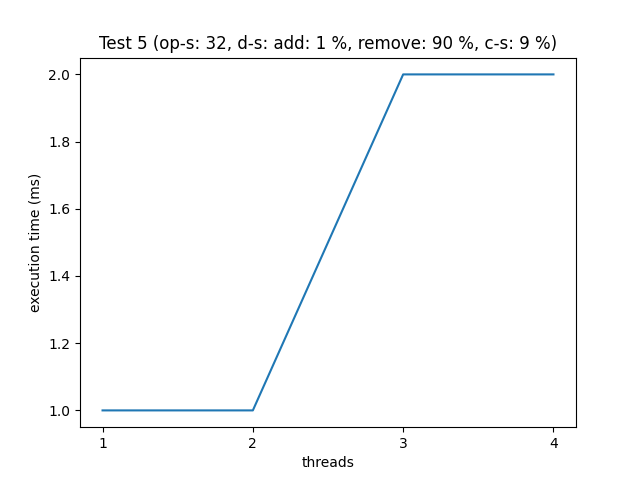
\includegraphics[width=0.7\linewidth]{photo/plot5}
    \caption{График результатов теста 5}
    \label{fig:plot5}
\end{figure}

\subsection*{Тест 6}

Параметры тестирования:

\begin{itemize}
    \item Количество операций: 32
    \item Вероятность выполнения операции \verb|add|: 9 \%
    \item Вероятность выполнения операции \verb|remove|: 1 \%
    \item Вероятность выполнения операции \verb|contains|: 90 \%
\end{itemize}

Результаты тестирования представленны в таблице \ref{tab:results6}


\begin{table}[H]
    \centering
    \begin{tabular}{|l|l|}
        \hline
        Кол-во потоков & Время выполнения (мс) \\
        \hline
        1 & 4 \\
        \hline
        2 & 4 \\
        \hline
        3 & 8 \\
        \hline
        4 & 5 \\
        \hline
    \end{tabular}
    \caption{Результаты теста 6}
    \label{tab:results6}
\end{table}
        

График результатов тестирования представлен на рис.\ref{fig:plot6}

\begin{figure}[H]
    \centering
    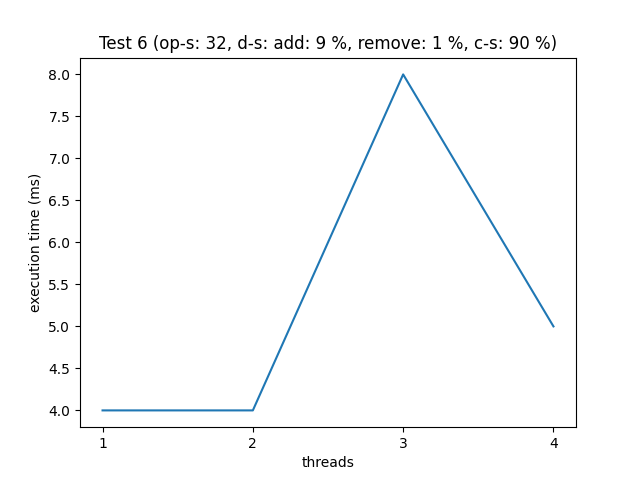
\includegraphics[width=0.7\linewidth]{photo/plot6}
    \caption{График результатов теста 6}
    \label{fig:plot6}
\end{figure}

\subsection*{Тест 7}

Параметры тестирования:

\begin{itemize}
    \item Количество операций: 32
    \item Вероятность выполнения операции \verb|add|: 1 \%
    \item Вероятность выполнения операции \verb|remove|: 9 \%
    \item Вероятность выполнения операции \verb|contains|: 90 \%
\end{itemize}

Результаты тестирования представленны в таблице \ref{tab:results7}


\begin{table}[H]
    \centering
    \begin{tabular}{|l|l|}
        \hline
        Кол-во потоков & Время выполнения (мс) \\
        \hline
        1 & 2 \\
        \hline
        2 & 4 \\
        \hline
        3 & 1 \\
        \hline
        4 & 1 \\
        \hline
    \end{tabular}
    \caption{Результаты теста 7}
    \label{tab:results7}
\end{table}
        

График результатов тестирования представлен на рис.\ref{fig:plot7}

\begin{figure}[H]
    \centering
    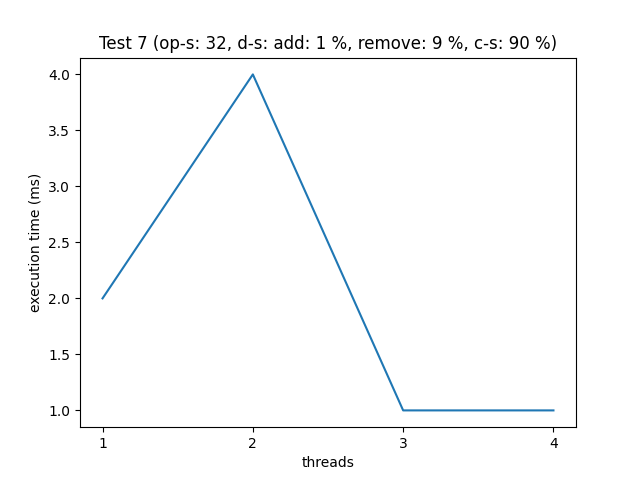
\includegraphics[width=0.7\linewidth]{photo/plot7}
    \caption{График результатов теста 7}
    \label{fig:plot7}
\end{figure}

\subsection*{Тест 8}

Параметры тестирования:

\begin{itemize}
    \item Количество операций: 128
    \item Вероятность выполнения операции \verb|add|: 33.33 \%
    \item Вероятность выполнения операции \verb|remove|: 33.33 \%
    \item Вероятность выполнения операции \verb|contains|: 33.33 \%
\end{itemize}

Результаты тестирования представленны в таблице \ref{tab:results8}


\begin{table}[H]
    \centering
    \begin{tabular}{|l|l|}
        \hline
        Кол-во потоков & Время выполнения (мс) \\
        \hline
        1 & 5 \\
        \hline
        2 & 9 \\
        \hline
        3 & 5 \\
        \hline
        4 & 4 \\
        \hline
    \end{tabular}
    \caption{Результаты теста 8}
    \label{tab:results8}
\end{table}
        

График результатов тестирования представлен на рис.\ref{fig:plot8}

\begin{figure}[H]
    \centering
    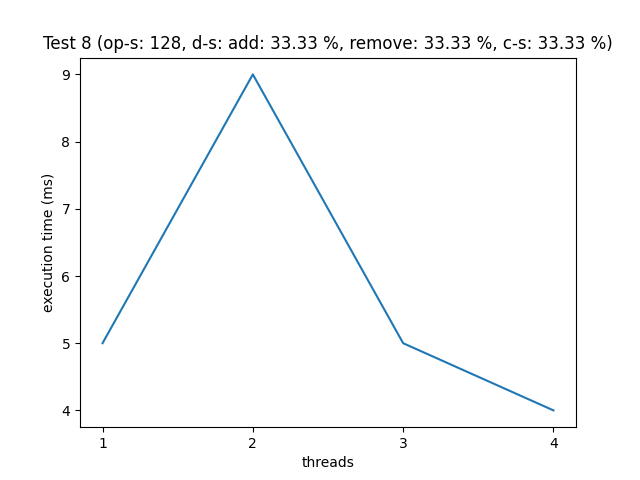
\includegraphics[width=0.7\linewidth]{photo/plot8}
    \caption{График результатов теста 8}
    \label{fig:plot8}
\end{figure}

\subsection*{Тест 9}

Параметры тестирования:

\begin{itemize}
    \item Количество операций: 128
    \item Вероятность выполнения операции \verb|add|: 90 \%
    \item Вероятность выполнения операции \verb|remove|: 9 \%
    \item Вероятность выполнения операции \verb|contains|: 1 \%
\end{itemize}

Результаты тестирования представленны в таблице \ref{tab:results9}


\begin{table}[H]
    \centering
    \begin{tabular}{|l|l|}
        \hline
        Кол-во потоков & Время выполнения (мс) \\
        \hline
        1 & 14 \\
        \hline
        2 & 3 \\
        \hline
        3 & 4 \\
        \hline
        4 & 6 \\
        \hline
    \end{tabular}
    \caption{Результаты теста 9}
    \label{tab:results9}
\end{table}
        

График результатов тестирования представлен на рис.\ref{fig:plot9}

\begin{figure}[H]
    \centering
    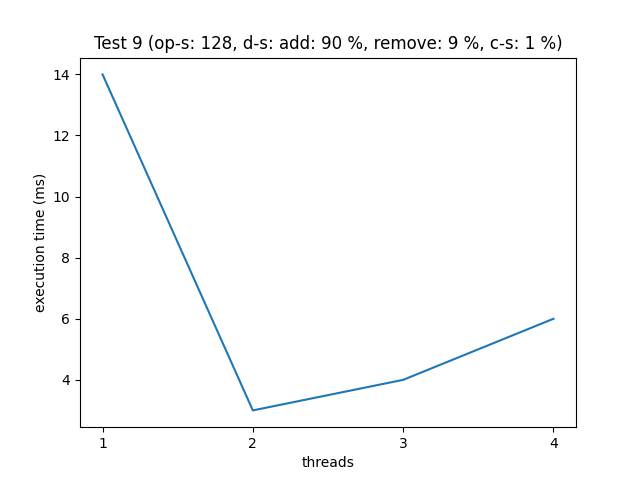
\includegraphics[width=0.7\linewidth]{photo/plot9}
    \caption{График результатов теста 9}
    \label{fig:plot9}
\end{figure}

\subsection*{Тест 10}

Параметры тестирования:

\begin{itemize}
    \item Количество операций: 128
    \item Вероятность выполнения операции \verb|add|: 90 \%
    \item Вероятность выполнения операции \verb|remove|: 1 \%
    \item Вероятность выполнения операции \verb|contains|: 9 \%
\end{itemize}

Результаты тестирования представленны в таблице \ref{tab:results10}


\begin{table}[H]
    \centering
    \begin{tabular}{|l|l|}
        \hline
        Кол-во потоков & Время выполнения (мс) \\
        \hline
        1 & 9 \\
        \hline
        2 & 7 \\
        \hline
        3 & 7 \\
        \hline
        4 & 3 \\
        \hline
    \end{tabular}
    \caption{Результаты теста 10}
    \label{tab:results10}
\end{table}
        

График результатов тестирования представлен на рис.\ref{fig:plot10}

\begin{figure}[H]
    \centering
    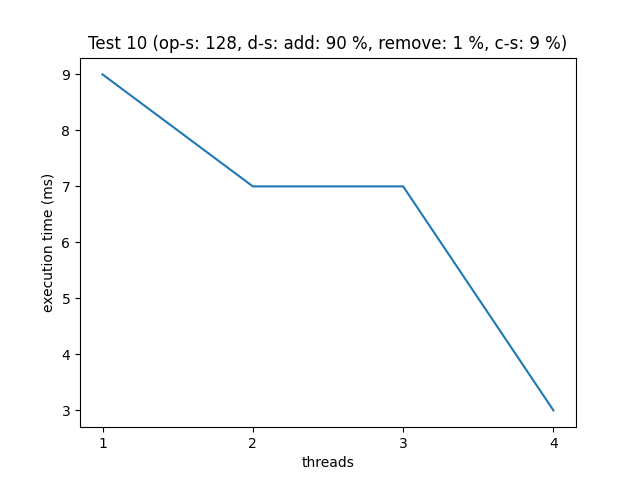
\includegraphics[width=0.7\linewidth]{photo/plot10}
    \caption{График результатов теста 10}
    \label{fig:plot10}
\end{figure}

\subsection*{Тест 11}

Параметры тестирования:

\begin{itemize}
    \item Количество операций: 128
    \item Вероятность выполнения операции \verb|add|: 9 \%
    \item Вероятность выполнения операции \verb|remove|: 90 \%
    \item Вероятность выполнения операции \verb|contains|: 1 \%
\end{itemize}

Результаты тестирования представленны в таблице \ref{tab:results11}


\begin{table}[H]
    \centering
    \begin{tabular}{|l|l|}
        \hline
        Кол-во потоков & Время выполнения (мс) \\
        \hline
        1 & 7 \\
        \hline
        2 & 5 \\
        \hline
        3 & 3 \\
        \hline
        4 & 39 \\
        \hline
    \end{tabular}
    \caption{Результаты теста 11}
    \label{tab:results11}
\end{table}
        

График результатов тестирования представлен на рис.\ref{fig:plot11}

\begin{figure}[H]
    \centering
    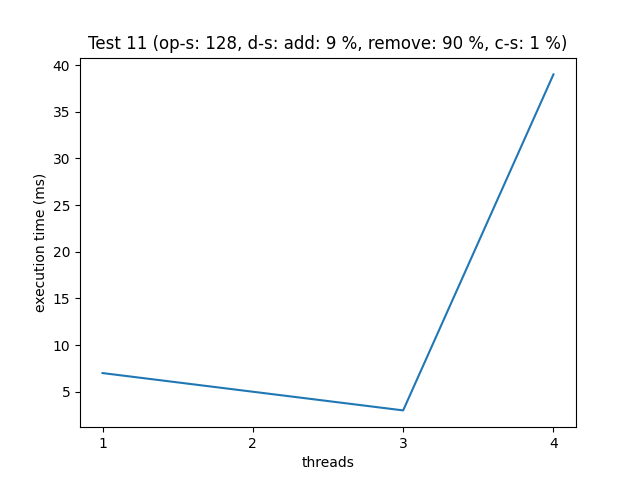
\includegraphics[width=0.7\linewidth]{photo/plot11}
    \caption{График результатов теста 11}
    \label{fig:plot11}
\end{figure}

\subsection*{Тест 12}

Параметры тестирования:

\begin{itemize}
    \item Количество операций: 128
    \item Вероятность выполнения операции \verb|add|: 1 \%
    \item Вероятность выполнения операции \verb|remove|: 90 \%
    \item Вероятность выполнения операции \verb|contains|: 9 \%
\end{itemize}

Результаты тестирования представленны в таблице \ref{tab:results12}


\begin{table}[H]
    \centering
    \begin{tabular}{|l|l|}
        \hline
        Кол-во потоков & Время выполнения (мс) \\
        \hline
        1 & 11 \\
        \hline
        2 & 4 \\
        \hline
        3 & 5 \\
        \hline
        4 & 4 \\
        \hline
    \end{tabular}
    \caption{Результаты теста 12}
    \label{tab:results12}
\end{table}
        

График результатов тестирования представлен на рис.\ref{fig:plot12}

\begin{figure}[H]
    \centering
    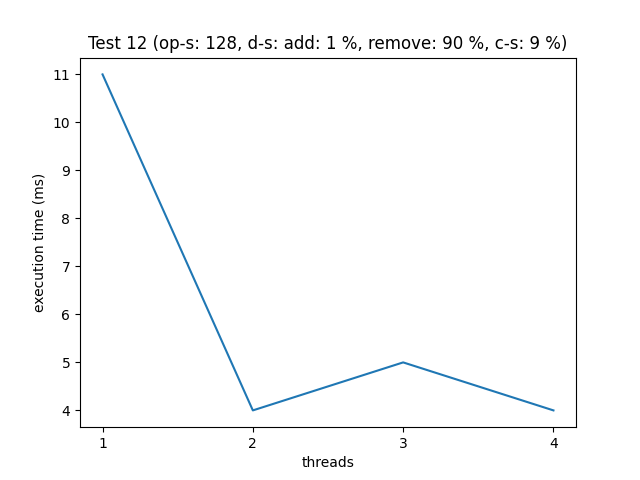
\includegraphics[width=0.7\linewidth]{photo/plot12}
    \caption{График результатов теста 12}
    \label{fig:plot12}
\end{figure}

\subsection*{Тест 13}

Параметры тестирования:

\begin{itemize}
    \item Количество операций: 128
    \item Вероятность выполнения операции \verb|add|: 9 \%
    \item Вероятность выполнения операции \verb|remove|: 1 \%
    \item Вероятность выполнения операции \verb|contains|: 90 \%
\end{itemize}

Результаты тестирования представленны в таблице \ref{tab:results13}


\begin{table}[H]
    \centering
    \begin{tabular}{|l|l|}
        \hline
        Кол-во потоков & Время выполнения (мс) \\
        \hline
        1 & 5 \\
        \hline
        2 & 13 \\
        \hline
        3 & 7 \\
        \hline
        4 & 6 \\
        \hline
    \end{tabular}
    \caption{Результаты теста 13}
    \label{tab:results13}
\end{table}
        

График результатов тестирования представлен на рис.\ref{fig:plot13}

\begin{figure}[H]
    \centering
    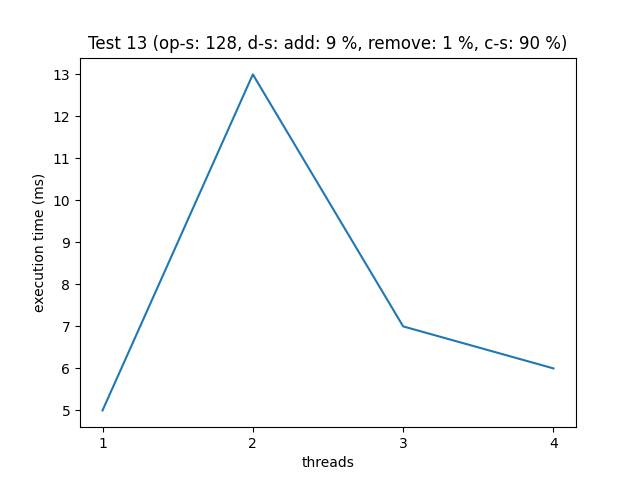
\includegraphics[width=0.7\linewidth]{photo/plot13}
    \caption{График результатов теста 13}
    \label{fig:plot13}
\end{figure}

\subsection*{Тест 14}

Параметры тестирования:

\begin{itemize}
    \item Количество операций: 128
    \item Вероятность выполнения операции \verb|add|: 1 \%
    \item Вероятность выполнения операции \verb|remove|: 9 \%
    \item Вероятность выполнения операции \verb|contains|: 90 \%
\end{itemize}

Результаты тестирования представленны в таблице \ref{tab:results14}


\begin{table}[H]
    \centering
    \begin{tabular}{|l|l|}
        \hline
        Кол-во потоков & Время выполнения (мс) \\
        \hline
        1 & 5 \\
        \hline
        2 & 2 \\
        \hline
        3 & 3 \\
        \hline
        4 & 12 \\
        \hline
    \end{tabular}
    \caption{Результаты теста 14}
    \label{tab:results14}
\end{table}
        

График результатов тестирования представлен на рис.\ref{fig:plot14}

\begin{figure}[H]
    \centering
    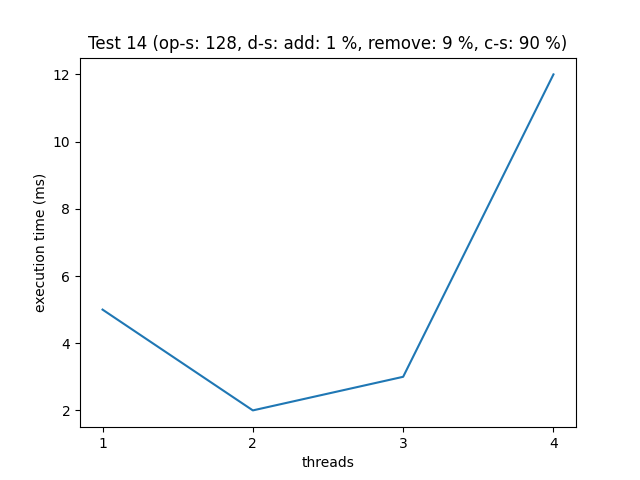
\includegraphics[width=0.7\linewidth]{photo/plot14}
    \caption{График результатов теста 14}
    \label{fig:plot14}
\end{figure}

\subsection*{Тест 15}

Параметры тестирования:

\begin{itemize}
    \item Количество операций: 1024
    \item Вероятность выполнения операции \verb|add|: 33.33 \%
    \item Вероятность выполнения операции \verb|remove|: 33.33 \%
    \item Вероятность выполнения операции \verb|contains|: 33.33 \%
\end{itemize}

Результаты тестирования представленны в таблице \ref{tab:results15}


\begin{table}[H]
    \centering
    \begin{tabular}{|l|l|}
        \hline
        Кол-во потоков & Время выполнения (мс) \\
        \hline
        1 & 49 \\
        \hline
        2 & 35 \\
        \hline
        3 & 46 \\
        \hline
        4 & 42 \\
        \hline
    \end{tabular}
    \caption{Результаты теста 15}
    \label{tab:results15}
\end{table}
        

График результатов тестирования представлен на рис.\ref{fig:plot15}

\begin{figure}[H]
    \centering
    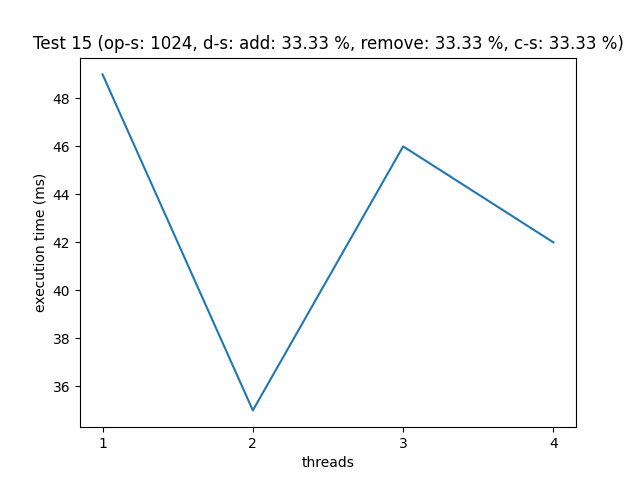
\includegraphics[width=0.7\linewidth]{photo/plot15}
    \caption{График результатов теста 15}
    \label{fig:plot15}
\end{figure}

\subsection*{Тест 16}

Параметры тестирования:

\begin{itemize}
    \item Количество операций: 1024
    \item Вероятность выполнения операции \verb|add|: 90 \%
    \item Вероятность выполнения операции \verb|remove|: 9 \%
    \item Вероятность выполнения операции \verb|contains|: 1 \%
\end{itemize}

Результаты тестирования представленны в таблице \ref{tab:results16}


\begin{table}[H]
    \centering
    \begin{tabular}{|l|l|}
        \hline
        Кол-во потоков & Время выполнения (мс) \\
        \hline
        1 & 80 \\
        \hline
        2 & 29 \\
        \hline
        3 & 24 \\
        \hline
        4 & 23 \\
        \hline
    \end{tabular}
    \caption{Результаты теста 16}
    \label{tab:results16}
\end{table}
        

График результатов тестирования представлен на рис.\ref{fig:plot16}

\begin{figure}[H]
    \centering
    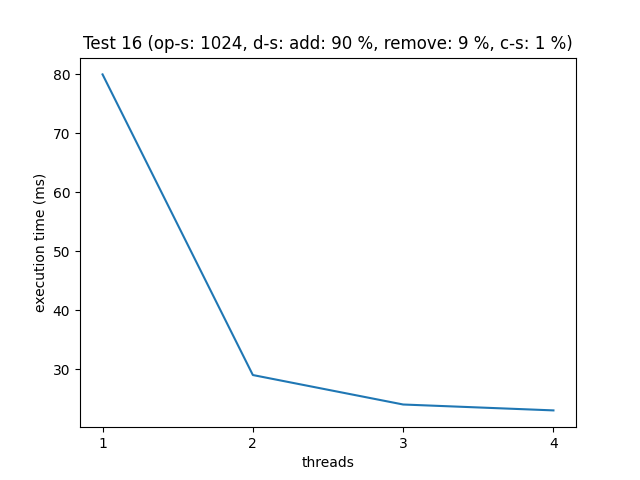
\includegraphics[width=0.7\linewidth]{photo/plot16}
    \caption{График результатов теста 16}
    \label{fig:plot16}
\end{figure}

\subsection*{Тест 17}

Параметры тестирования:

\begin{itemize}
    \item Количество операций: 1024
    \item Вероятность выполнения операции \verb|add|: 90 \%
    \item Вероятность выполнения операции \verb|remove|: 1 \%
    \item Вероятность выполнения операции \verb|contains|: 9 \%
\end{itemize}

Результаты тестирования представленны в таблице \ref{tab:results17}


\begin{table}[H]
    \centering
    \begin{tabular}{|l|l|}
        \hline
        Кол-во потоков & Время выполнения (мс) \\
        \hline
        1 & 46 \\
        \hline
        2 & 30 \\
        \hline
        3 & 22 \\
        \hline
        4 & 19 \\
        \hline
    \end{tabular}
    \caption{Результаты теста 17}
    \label{tab:results17}
\end{table}
        

График результатов тестирования представлен на рис.\ref{fig:plot17}

\begin{figure}[H]
    \centering
    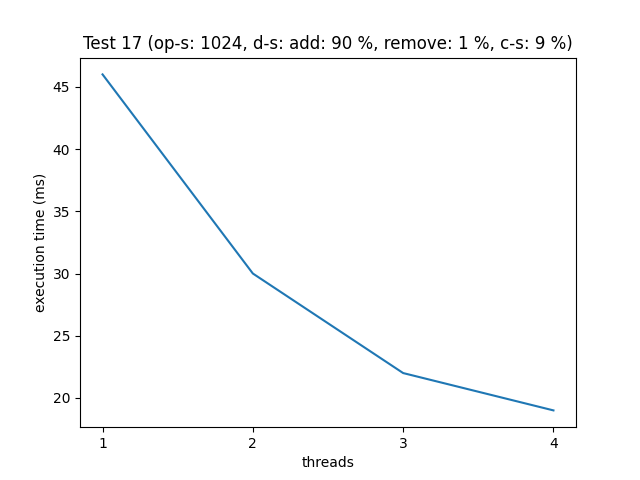
\includegraphics[width=0.7\linewidth]{photo/plot17}
    \caption{График результатов теста 17}
    \label{fig:plot17}
\end{figure}

\subsection*{Тест 18}

Параметры тестирования:

\begin{itemize}
    \item Количество операций: 1024
    \item Вероятность выполнения операции \verb|add|: 9 \%
    \item Вероятность выполнения операции \verb|remove|: 90 \%
    \item Вероятность выполнения операции \verb|contains|: 1 \%
\end{itemize}

Результаты тестирования представленны в таблице \ref{tab:results18}


\begin{table}[H]
    \centering
    \begin{tabular}{|l|l|}
        \hline
        Кол-во потоков & Время выполнения (мс) \\
        \hline
        1 & 43 \\
        \hline
        2 & 27 \\
        \hline
        3 & 22 \\
        \hline
        4 & 30 \\
        \hline
    \end{tabular}
    \caption{Результаты теста 18}
    \label{tab:results18}
\end{table}
        

График результатов тестирования представлен на рис.\ref{fig:plot18}

\begin{figure}[H]
    \centering
    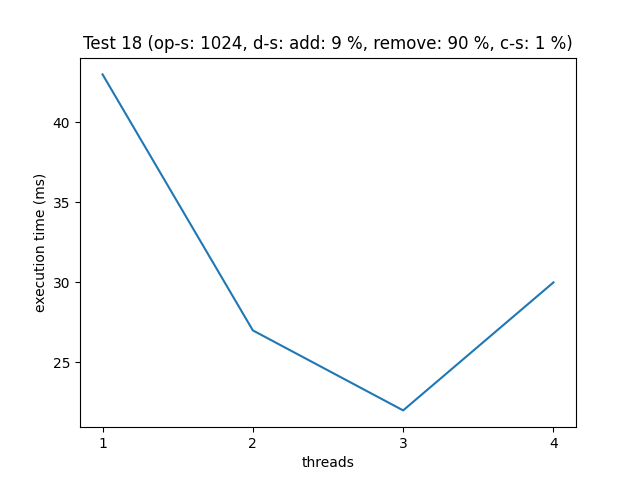
\includegraphics[width=0.7\linewidth]{photo/plot18}
    \caption{График результатов теста 18}
    \label{fig:plot18}
\end{figure}

\subsection*{Тест 19}

Параметры тестирования:

\begin{itemize}
    \item Количество операций: 1024
    \item Вероятность выполнения операции \verb|add|: 1 \%
    \item Вероятность выполнения операции \verb|remove|: 90 \%
    \item Вероятность выполнения операции \verb|contains|: 9 \%
\end{itemize}

Результаты тестирования представленны в таблице \ref{tab:results19}


\begin{table}[H]
    \centering
    \begin{tabular}{|l|l|}
        \hline
        Кол-во потоков & Время выполнения (мс) \\
        \hline
        1 & 50 \\
        \hline
        2 & 39 \\
        \hline
        3 & 22 \\
        \hline
        4 & 23 \\
        \hline
    \end{tabular}
    \caption{Результаты теста 19}
    \label{tab:results19}
\end{table}
        

График результатов тестирования представлен на рис.\ref{fig:plot19}

\begin{figure}[H]
    \centering
    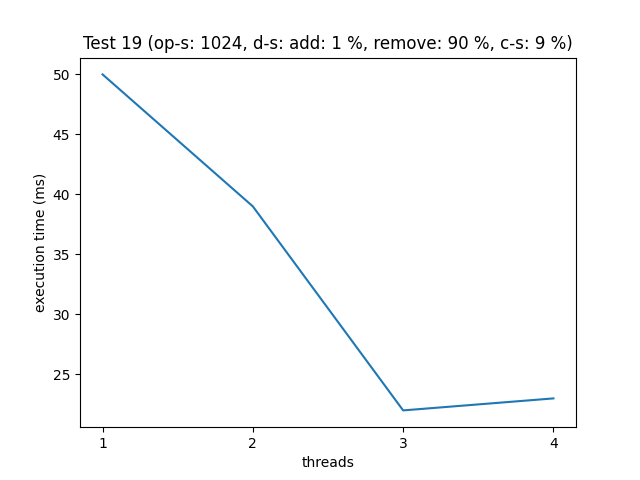
\includegraphics[width=0.7\linewidth]{photo/plot19}
    \caption{График результатов теста 19}
    \label{fig:plot19}
\end{figure}

\subsection*{Тест 20}

Параметры тестирования:

\begin{itemize}
    \item Количество операций: 1024
    \item Вероятность выполнения операции \verb|add|: 9 \%
    \item Вероятность выполнения операции \verb|remove|: 1 \%
    \item Вероятность выполнения операции \verb|contains|: 90 \%
\end{itemize}

Результаты тестирования представленны в таблице \ref{tab:results20}


\begin{table}[H]
    \centering
    \begin{tabular}{|l|l|}
        \hline
        Кол-во потоков & Время выполнения (мс) \\
        \hline
        1 & 44 \\
        \hline
        2 & 37 \\
        \hline
        3 & 21 \\
        \hline
        4 & 34 \\
        \hline
    \end{tabular}
    \caption{Результаты теста 20}
    \label{tab:results20}
\end{table}
        

График результатов тестирования представлен на рис.\ref{fig:plot20}

\begin{figure}[H]
    \centering
    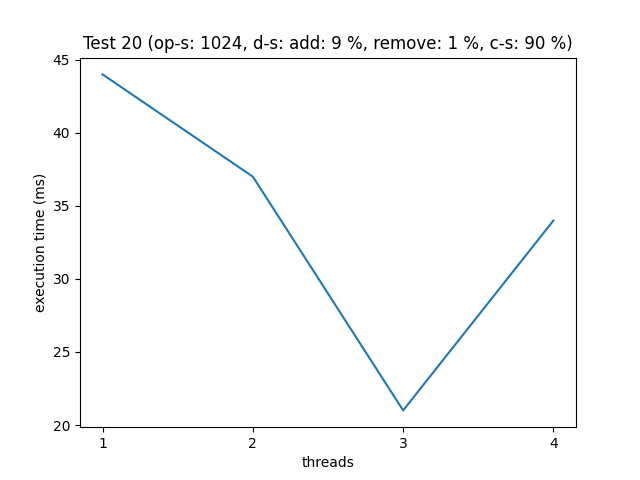
\includegraphics[width=0.7\linewidth]{photo/plot20}
    \caption{График результатов теста 20}
    \label{fig:plot20}
\end{figure}

\subsection*{Тест 21}

Параметры тестирования:

\begin{itemize}
    \item Количество операций: 1024
    \item Вероятность выполнения операции \verb|add|: 1 \%
    \item Вероятность выполнения операции \verb|remove|: 9 \%
    \item Вероятность выполнения операции \verb|contains|: 90 \%
\end{itemize}

Результаты тестирования представленны в таблице \ref{tab:results21}


\begin{table}[H]
    \centering
    \begin{tabular}{|l|l|}
        \hline
        Кол-во потоков & Время выполнения (мс) \\
        \hline
        1 & 43 \\
        \hline
        2 & 26 \\
        \hline
        3 & 24 \\
        \hline
        4 & 21 \\
        \hline
    \end{tabular}
    \caption{Результаты теста 21}
    \label{tab:results21}
\end{table}
        

График результатов тестирования представлен на рис.\ref{fig:plot21}

\begin{figure}[H]
    \centering
    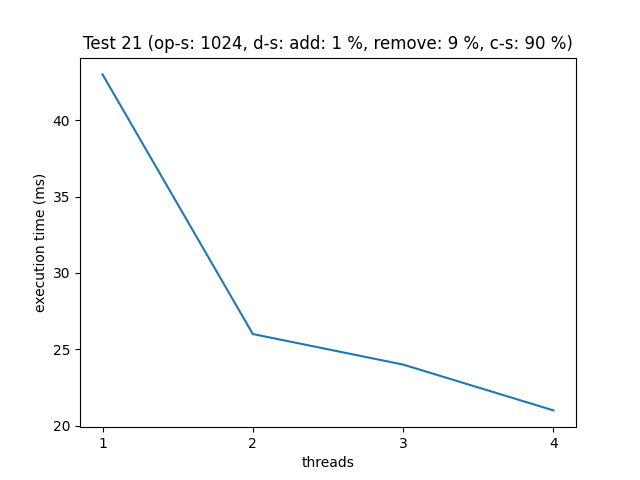
\includegraphics[width=0.7\linewidth]{photo/plot21}
    \caption{График результатов теста 21}
    \label{fig:plot21}
\end{figure}

\subsection*{Тест 22}

Параметры тестирования:

\begin{itemize}
    \item Количество операций: 32768
    \item Вероятность выполнения операции \verb|add|: 33.33 \%
    \item Вероятность выполнения операции \verb|remove|: 33.33 \%
    \item Вероятность выполнения операции \verb|contains|: 33.33 \%
\end{itemize}

Результаты тестирования представленны в таблице \ref{tab:results22}


\begin{table}[H]
    \centering
    \begin{tabular}{|l|l|}
        \hline
        Кол-во потоков & Время выполнения (мс) \\
        \hline
        1 & 1350 \\
        \hline
        2 & 828 \\
        \hline
        3 & 599 \\
        \hline
        4 & 605 \\
        \hline
    \end{tabular}
    \caption{Результаты теста 22}
    \label{tab:results22}
\end{table}
        

График результатов тестирования представлен на рис.\ref{fig:plot22}

\begin{figure}[H]
    \centering
    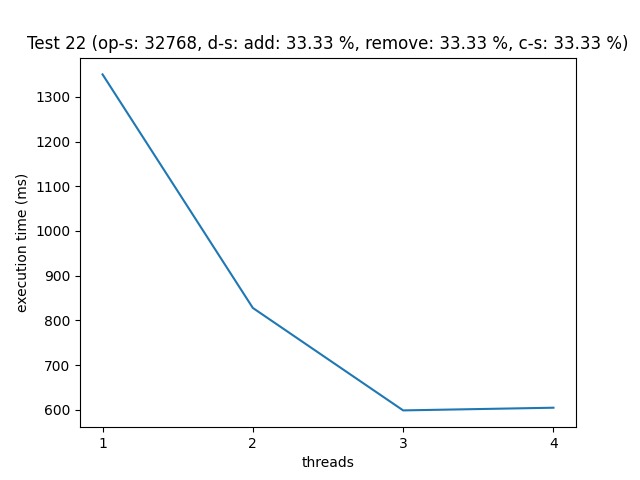
\includegraphics[width=0.7\linewidth]{photo/plot22}
    \caption{График результатов теста 22}
    \label{fig:plot22}
\end{figure}

\subsection*{Тест 23}

Параметры тестирования:

\begin{itemize}
    \item Количество операций: 32768
    \item Вероятность выполнения операции \verb|add|: 90 \%
    \item Вероятность выполнения операции \verb|remove|: 9 \%
    \item Вероятность выполнения операции \verb|contains|: 1 \%
\end{itemize}

Результаты тестирования представленны в таблице \ref{tab:results23}


\begin{table}[H]
    \centering
    \begin{tabular}{|l|l|}
        \hline
        Кол-во потоков & Время выполнения (мс) \\
        \hline
        1 & 1399 \\
        \hline
        2 & 724 \\
        \hline
        3 & 582 \\
        \hline
        4 & 567 \\
        \hline
    \end{tabular}
    \caption{Результаты теста 23}
    \label{tab:results23}
\end{table}
        

График результатов тестирования представлен на рис.\ref{fig:plot23}

\begin{figure}[H]
    \centering
    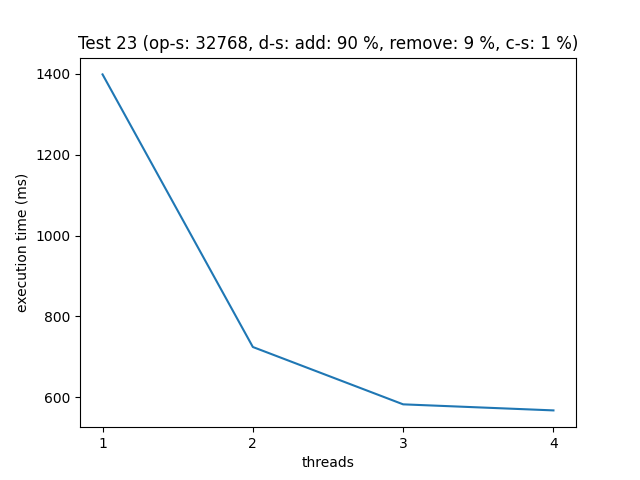
\includegraphics[width=0.7\linewidth]{photo/plot23}
    \caption{График результатов теста 23}
    \label{fig:plot23}
\end{figure}

\subsection*{Тест 24}

Параметры тестирования:

\begin{itemize}
    \item Количество операций: 32768
    \item Вероятность выполнения операции \verb|add|: 90 \%
    \item Вероятность выполнения операции \verb|remove|: 1 \%
    \item Вероятность выполнения операции \verb|contains|: 9 \%
\end{itemize}

Результаты тестирования представленны в таблице \ref{tab:results24}


\begin{table}[H]
    \centering
    \begin{tabular}{|l|l|}
        \hline
        Кол-во потоков & Время выполнения (мс) \\
        \hline
        1 & 1414 \\
        \hline
        2 & 825 \\
        \hline
        3 & 596 \\
        \hline
        4 & 580 \\
        \hline
    \end{tabular}
    \caption{Результаты теста 24}
    \label{tab:results24}
\end{table}
        

График результатов тестирования представлен на рис.\ref{fig:plot24}

\begin{figure}[H]
    \centering
    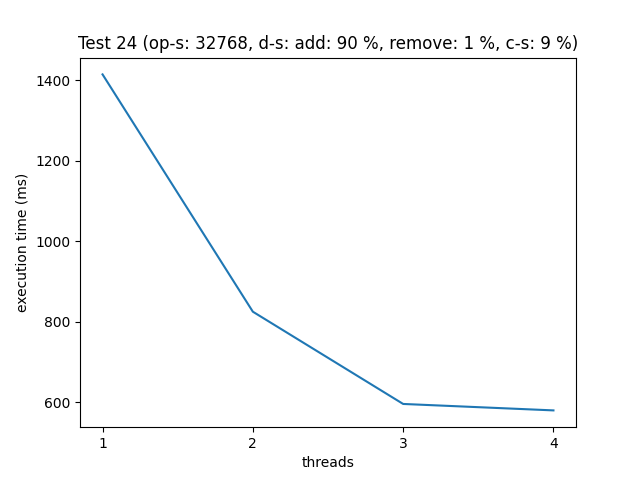
\includegraphics[width=0.7\linewidth]{photo/plot24}
    \caption{График результатов теста 24}
    \label{fig:plot24}
\end{figure}

\subsection*{Тест 25}

Параметры тестирования:

\begin{itemize}
    \item Количество операций: 32768
    \item Вероятность выполнения операции \verb|add|: 9 \%
    \item Вероятность выполнения операции \verb|remove|: 90 \%
    \item Вероятность выполнения операции \verb|contains|: 1 \%
\end{itemize}

Результаты тестирования представленны в таблице \ref{tab:results25}


\begin{table}[H]
    \centering
    \begin{tabular}{|l|l|}
        \hline
        Кол-во потоков & Время выполнения (мс) \\
        \hline
        1 & 1319 \\
        \hline
        2 & 675 \\
        \hline
        3 & 562 \\
        \hline
        4 & 554 \\
        \hline
    \end{tabular}
    \caption{Результаты теста 25}
    \label{tab:results25}
\end{table}
        

График результатов тестирования представлен на рис.\ref{fig:plot25}

\begin{figure}[H]
    \centering
    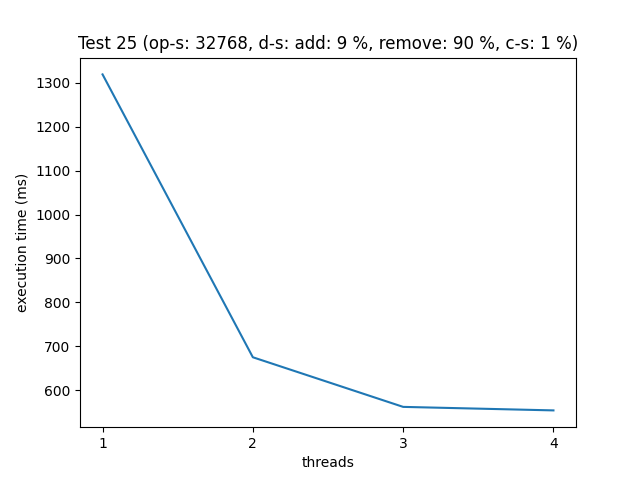
\includegraphics[width=0.7\linewidth]{photo/plot25}
    \caption{График результатов теста 25}
    \label{fig:plot25}
\end{figure}

\subsection*{Тест 26}

Параметры тестирования:

\begin{itemize}
    \item Количество операций: 32768
    \item Вероятность выполнения операции \verb|add|: 1 \%
    \item Вероятность выполнения операции \verb|remove|: 90 \%
    \item Вероятность выполнения операции \verb|contains|: 9 \%
\end{itemize}

Результаты тестирования представленны в таблице \ref{tab:results26}


\begin{table}[H]
    \centering
    \begin{tabular}{|l|l|}
        \hline
        Кол-во потоков & Время выполнения (мс) \\
        \hline
        1 & 1304 \\
        \hline
        2 & 681 \\
        \hline
        3 & 554 \\
        \hline
        4 & 554 \\
        \hline
    \end{tabular}
    \caption{Результаты теста 26}
    \label{tab:results26}
\end{table}
        

График результатов тестирования представлен на рис.\ref{fig:plot26}

\begin{figure}[H]
    \centering
    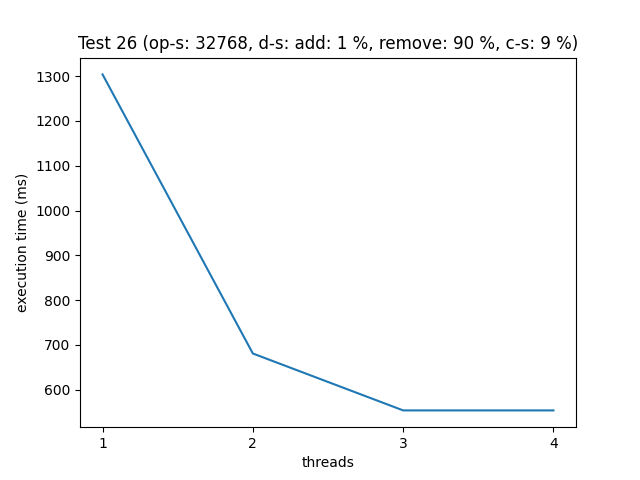
\includegraphics[width=0.7\linewidth]{photo/plot26}
    \caption{График результатов теста 26}
    \label{fig:plot26}
\end{figure}

\subsection*{Тест 27}

Параметры тестирования:

\begin{itemize}
    \item Количество операций: 32768
    \item Вероятность выполнения операции \verb|add|: 9 \%
    \item Вероятность выполнения операции \verb|remove|: 1 \%
    \item Вероятность выполнения операции \verb|contains|: 90 \%
\end{itemize}

Результаты тестирования представленны в таблице \ref{tab:results27}


\begin{table}[H]
    \centering
    \begin{tabular}{|l|l|}
        \hline
        Кол-во потоков & Время выполнения (мс) \\
        \hline
        1 & 1360 \\
        \hline
        2 & 775 \\
        \hline
        3 & 623 \\
        \hline
        4 & 553 \\
        \hline
    \end{tabular}
    \caption{Результаты теста 27}
    \label{tab:results27}
\end{table}
        

График результатов тестирования представлен на рис.\ref{fig:plot27}

\begin{figure}[H]
    \centering
    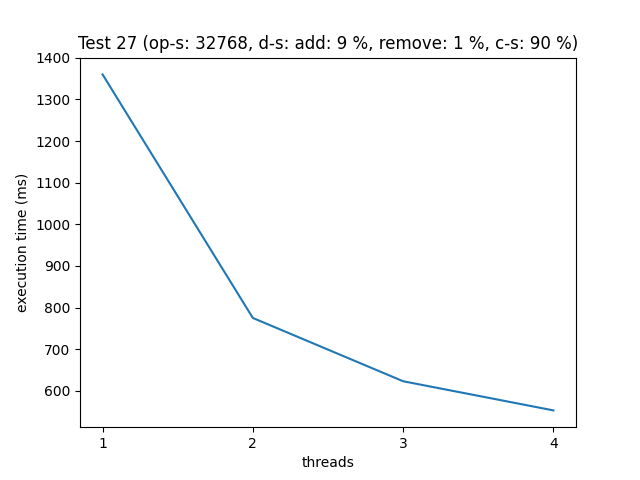
\includegraphics[width=0.7\linewidth]{photo/plot27}
    \caption{График результатов теста 27}
    \label{fig:plot27}
\end{figure}

\subsection*{Тест 28}

Параметры тестирования:

\begin{itemize}
    \item Количество операций: 32768
    \item Вероятность выполнения операции \verb|add|: 1 \%
    \item Вероятность выполнения операции \verb|remove|: 9 \%
    \item Вероятность выполнения операции \verb|contains|: 90 \%
\end{itemize}

Результаты тестирования представленны в таблице \ref{tab:results28}


\begin{table}[H]
    \centering
    \begin{tabular}{|l|l|}
        \hline
        Кол-во потоков & Время выполнения (мс) \\
        \hline
        1 & 1312 \\
        \hline
        2 & 671 \\
        \hline
        3 & 549 \\
        \hline
        4 & 533 \\
        \hline
    \end{tabular}
    \caption{Результаты теста 28}
    \label{tab:results28}
\end{table}
        

График результатов тестирования представлен на рис.\ref{fig:plot28}

\begin{figure}[H]
    \centering
    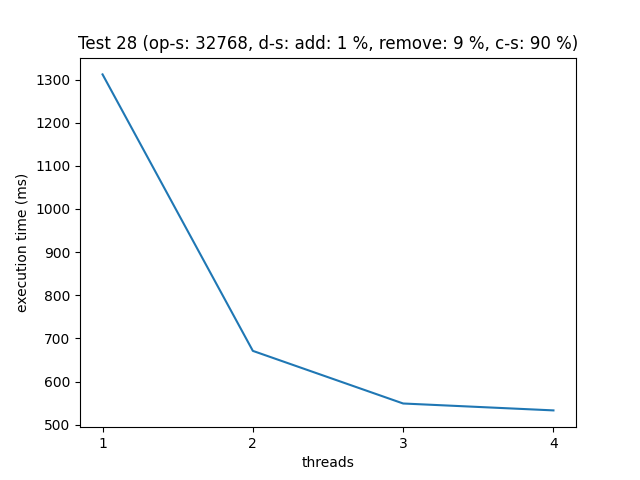
\includegraphics[width=0.7\linewidth]{photo/plot28}
    \caption{График результатов теста 28}
    \label{fig:plot28}
\end{figure}

\subsection*{Тест 29}

Параметры тестирования:

\begin{itemize}
    \item Количество операций: 131072
    \item Вероятность выполнения операции \verb|add|: 33.33 \%
    \item Вероятность выполнения операции \verb|remove|: 33.33 \%
    \item Вероятность выполнения операции \verb|contains|: 33.33 \%
\end{itemize}

Результаты тестирования представленны в таблице \ref{tab:results29}


\begin{table}[H]
    \centering
    \begin{tabular}{|l|l|}
        \hline
        Кол-во потоков & Время выполнения (мс) \\
        \hline
        1 & 5351 \\
        \hline
        2 & 2721 \\
        \hline
        3 & 2149 \\
        \hline
        4 & 2094 \\
        \hline
    \end{tabular}
    \caption{Результаты теста 29}
    \label{tab:results29}
\end{table}
        

График результатов тестирования представлен на рис.\ref{fig:plot29}

\begin{figure}[H]
    \centering
    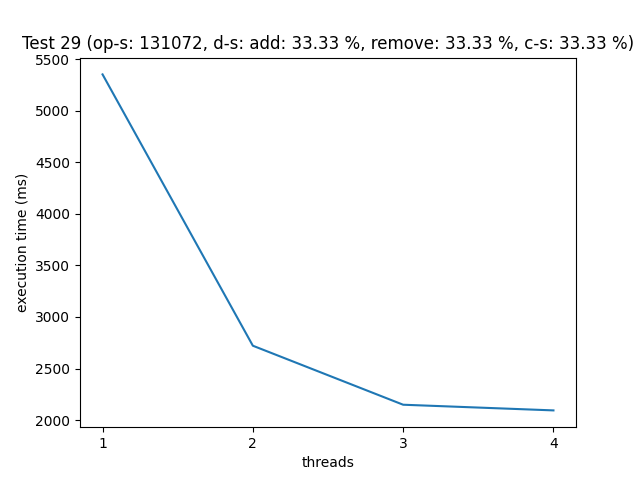
\includegraphics[width=0.7\linewidth]{photo/plot29}
    \caption{График результатов теста 29}
    \label{fig:plot29}
\end{figure}

\subsection*{Тест 30}

Параметры тестирования:

\begin{itemize}
    \item Количество операций: 131072
    \item Вероятность выполнения операции \verb|add|: 90 \%
    \item Вероятность выполнения операции \verb|remove|: 9 \%
    \item Вероятность выполнения операции \verb|contains|: 1 \%
\end{itemize}

Результаты тестирования представленны в таблице \ref{tab:results30}


\begin{table}[H]
    \centering
    \begin{tabular}{|l|l|}
        \hline
        Кол-во потоков & Время выполнения (мс) \\
        \hline
        1 & 5531 \\
        \hline
        2 & 2834 \\
        \hline
        3 & 2198 \\
        \hline
        4 & 2122 \\
        \hline
    \end{tabular}
    \caption{Результаты теста 30}
    \label{tab:results30}
\end{table}
        

График результатов тестирования представлен на рис.\ref{fig:plot30}

\begin{figure}[H]
    \centering
    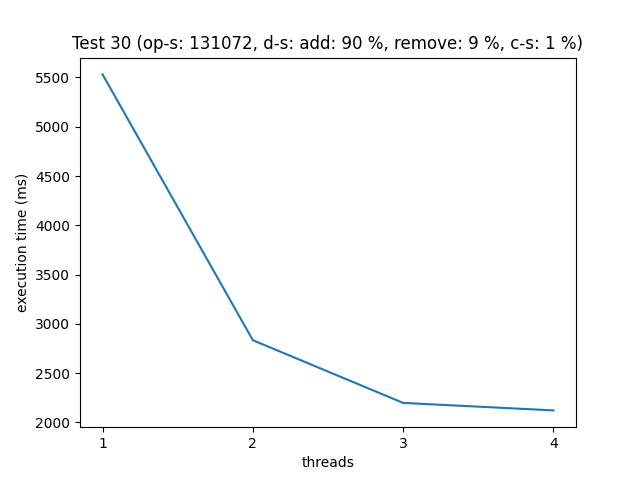
\includegraphics[width=0.7\linewidth]{photo/plot30}
    \caption{График результатов теста 30}
    \label{fig:plot30}
\end{figure}

\subsection*{Тест 31}

Параметры тестирования:

\begin{itemize}
    \item Количество операций: 131072
    \item Вероятность выполнения операции \verb|add|: 90 \%
    \item Вероятность выполнения операции \verb|remove|: 1 \%
    \item Вероятность выполнения операции \verb|contains|: 9 \%
\end{itemize}

Результаты тестирования представленны в таблице \ref{tab:results31}


\begin{table}[H]
    \centering
    \begin{tabular}{|l|l|}
        \hline
        Кол-во потоков & Время выполнения (мс) \\
        \hline
        1 & 5546 \\
        \hline
        2 & 2816 \\
        \hline
        3 & 2204 \\
        \hline
        4 & 2125 \\
        \hline
    \end{tabular}
    \caption{Результаты теста 31}
    \label{tab:results31}
\end{table}
        

График результатов тестирования представлен на рис.\ref{fig:plot31}

\begin{figure}[H]
    \centering
    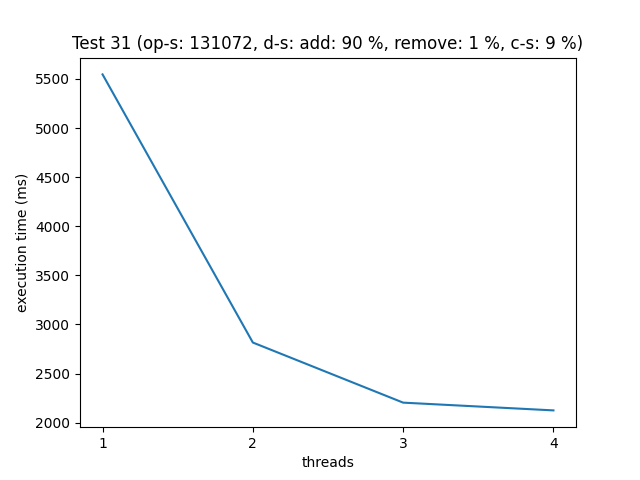
\includegraphics[width=0.7\linewidth]{photo/plot31}
    \caption{График результатов теста 31}
    \label{fig:plot31}
\end{figure}

\subsection*{Тест 32}

Параметры тестирования:

\begin{itemize}
    \item Количество операций: 131072
    \item Вероятность выполнения операции \verb|add|: 9 \%
    \item Вероятность выполнения операции \verb|remove|: 90 \%
    \item Вероятность выполнения операции \verb|contains|: 1 \%
\end{itemize}

Результаты тестирования представленны в таблице \ref{tab:results32}


\begin{table}[H]
    \centering
    \begin{tabular}{|l|l|}
        \hline
        Кол-во потоков & Время выполнения (мс) \\
        \hline
        1 & 5211 \\
        \hline
        2 & 2671 \\
        \hline
        3 & 2128 \\
        \hline
        4 & 2091 \\
        \hline
    \end{tabular}
    \caption{Результаты теста 32}
    \label{tab:results32}
\end{table}
        

График результатов тестирования представлен на рис.\ref{fig:plot32}

\begin{figure}[H]
    \centering
    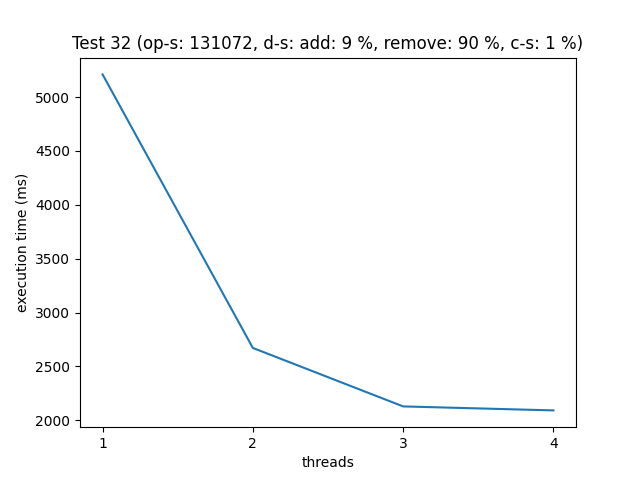
\includegraphics[width=0.7\linewidth]{photo/plot32}
    \caption{График результатов теста 32}
    \label{fig:plot32}
\end{figure}

\subsection*{Тест 33}

Параметры тестирования:

\begin{itemize}
    \item Количество операций: 131072
    \item Вероятность выполнения операции \verb|add|: 1 \%
    \item Вероятность выполнения операции \verb|remove|: 90 \%
    \item Вероятность выполнения операции \verb|contains|: 9 \%
\end{itemize}

Результаты тестирования представленны в таблице \ref{tab:results33}


\begin{table}[H]
    \centering
    \begin{tabular}{|l|l|}
        \hline
        Кол-во потоков & Время выполнения (мс) \\
        \hline
        1 & 5191 \\
        \hline
        2 & 2630 \\
        \hline
        3 & 2119 \\
        \hline
        4 & 2100 \\
        \hline
    \end{tabular}
    \caption{Результаты теста 33}
    \label{tab:results33}
\end{table}
        

График результатов тестирования представлен на рис.\ref{fig:plot33}

\begin{figure}[H]
    \centering
    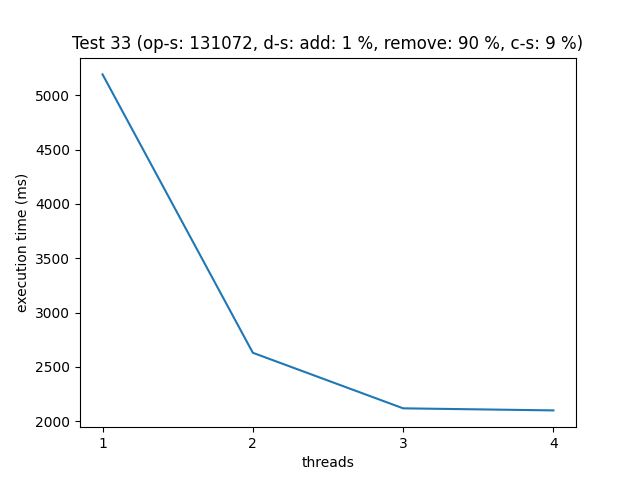
\includegraphics[width=0.7\linewidth]{photo/plot33}
    \caption{График результатов теста 33}
    \label{fig:plot33}
\end{figure}

\subsection*{Тест 34}

Параметры тестирования:

\begin{itemize}
    \item Количество операций: 131072
    \item Вероятность выполнения операции \verb|add|: 9 \%
    \item Вероятность выполнения операции \verb|remove|: 1 \%
    \item Вероятность выполнения операции \verb|contains|: 90 \%
\end{itemize}

Результаты тестирования представленны в таблице \ref{tab:results34}


\begin{table}[H]
    \centering
    \begin{tabular}{|l|l|}
        \hline
        Кол-во потоков & Время выполнения (мс) \\
        \hline
        1 & 5486 \\
        \hline
        2 & 2833 \\
        \hline
        3 & 2194 \\
        \hline
        4 & 2103 \\
        \hline
    \end{tabular}
    \caption{Результаты теста 34}
    \label{tab:results34}
\end{table}
        

График результатов тестирования представлен на рис.\ref{fig:plot34}

\begin{figure}[H]
    \centering
    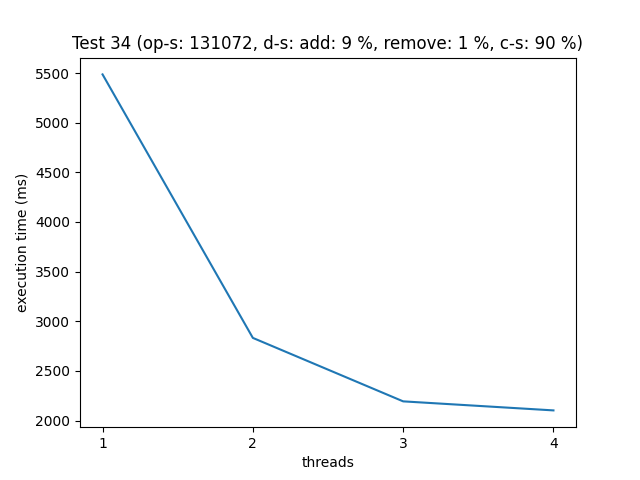
\includegraphics[width=0.7\linewidth]{photo/plot34}
    \caption{График результатов теста 34}
    \label{fig:plot34}
\end{figure}

\subsection*{Тест 35}

Параметры тестирования:

\begin{itemize}
    \item Количество операций: 131072
    \item Вероятность выполнения операции \verb|add|: 1 \%
    \item Вероятность выполнения операции \verb|remove|: 9 \%
    \item Вероятность выполнения операции \verb|contains|: 90 \%
\end{itemize}

Результаты тестирования представленны в таблице \ref{tab:results35}


\begin{table}[H]
    \centering
    \begin{tabular}{|l|l|}
        \hline
        Кол-во потоков & Время выполнения (мс) \\
        \hline
        1 & 5209 \\
        \hline
        2 & 2688 \\
        \hline
        3 & 2157 \\
        \hline
        4 & 2083 \\
        \hline
    \end{tabular}
    \caption{Результаты теста 35}
    \label{tab:results35}
\end{table}
        

График результатов тестирования представлен на рис.\ref{fig:plot35}

\begin{figure}[H]
    \centering
    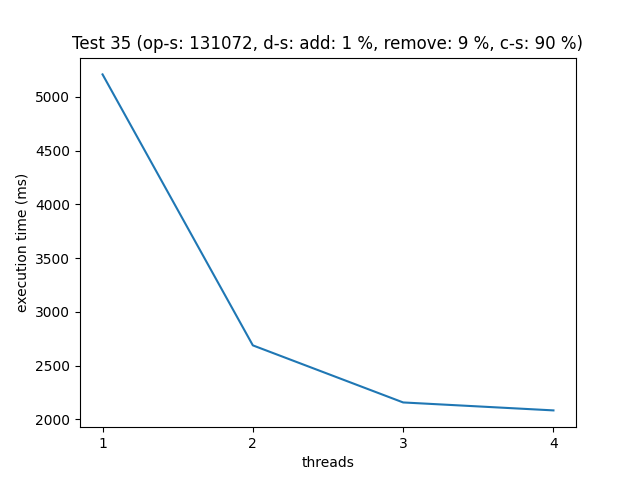
\includegraphics[width=0.7\linewidth]{photo/plot35}
    \caption{График результатов теста 35}
    \label{fig:plot35}
\end{figure}